\section{PPF Design and Architecture}
\label{Arch}

\begin{figure}
  \begin{center}
  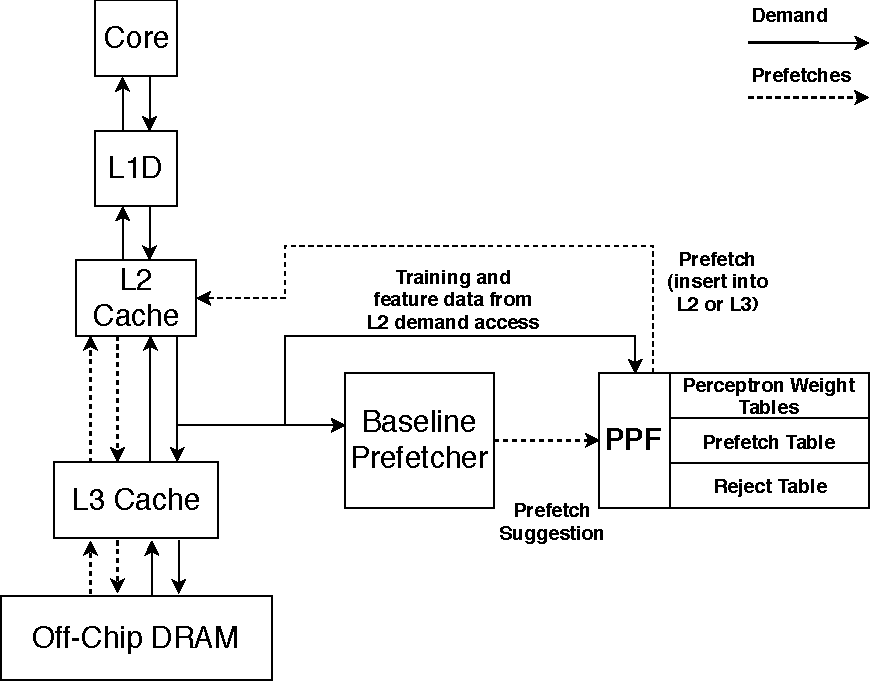
\includegraphics[width=8cm]{PPF_Hierarchy}
  \caption{PPF Architecture in the Memory Hierarchy}
  \label{fig:PPF_Hierarchy}
  \end{center}
\end{figure}

It can be beneficial to allow a prefetcher to speculate as deeply as
possible. Often, some useful prefetches are generated long after the
confidence of the prefetcher has fallen below the point at which
performance degrades due to the increase of inaccurate prefetches.  In
order to allow deep speculation in the prefetcher, however, inaccurate
prefetches must be filtered out.  We propose to leverage
perceptron-based learning as a mechanism to differentiate between
potentially useful deeply speculated prefetches and likely not-useful
ones. The Perceptron Prefetch Filter (PPF) is placed between the
prefetcher and the prefetch insertion queue, as illustrated in
Figure~\ref{fig:PPF_Hierarchy}, to prevent not-useful prefetches from
polluting the higher levels of the memory hierarchy.

Perceptron learning is a light-weight mechanism to pull together
disparate forms of information and synthesize a decision from
them. Our work considers a number of features corresponding to a
prefetch, such as speculation depth, page address and offset, and uses
this information as the inputs to our perceptron-based filter in order
to predict the usefulness of a prefetch.  Here, we discuss our the
design of our proposed perceptron prefetch filter (PPF).  PPF enhances
{an underlying prefetcher} by filtering out predicted unused prefetches. 
PPF is a generalized prefetch filtering mechanism that may be adapted 
to any prefetcher with appropriate feature selection and modifications 
which we describe below.

\begin{figure}[ht]
  \begin{center}
  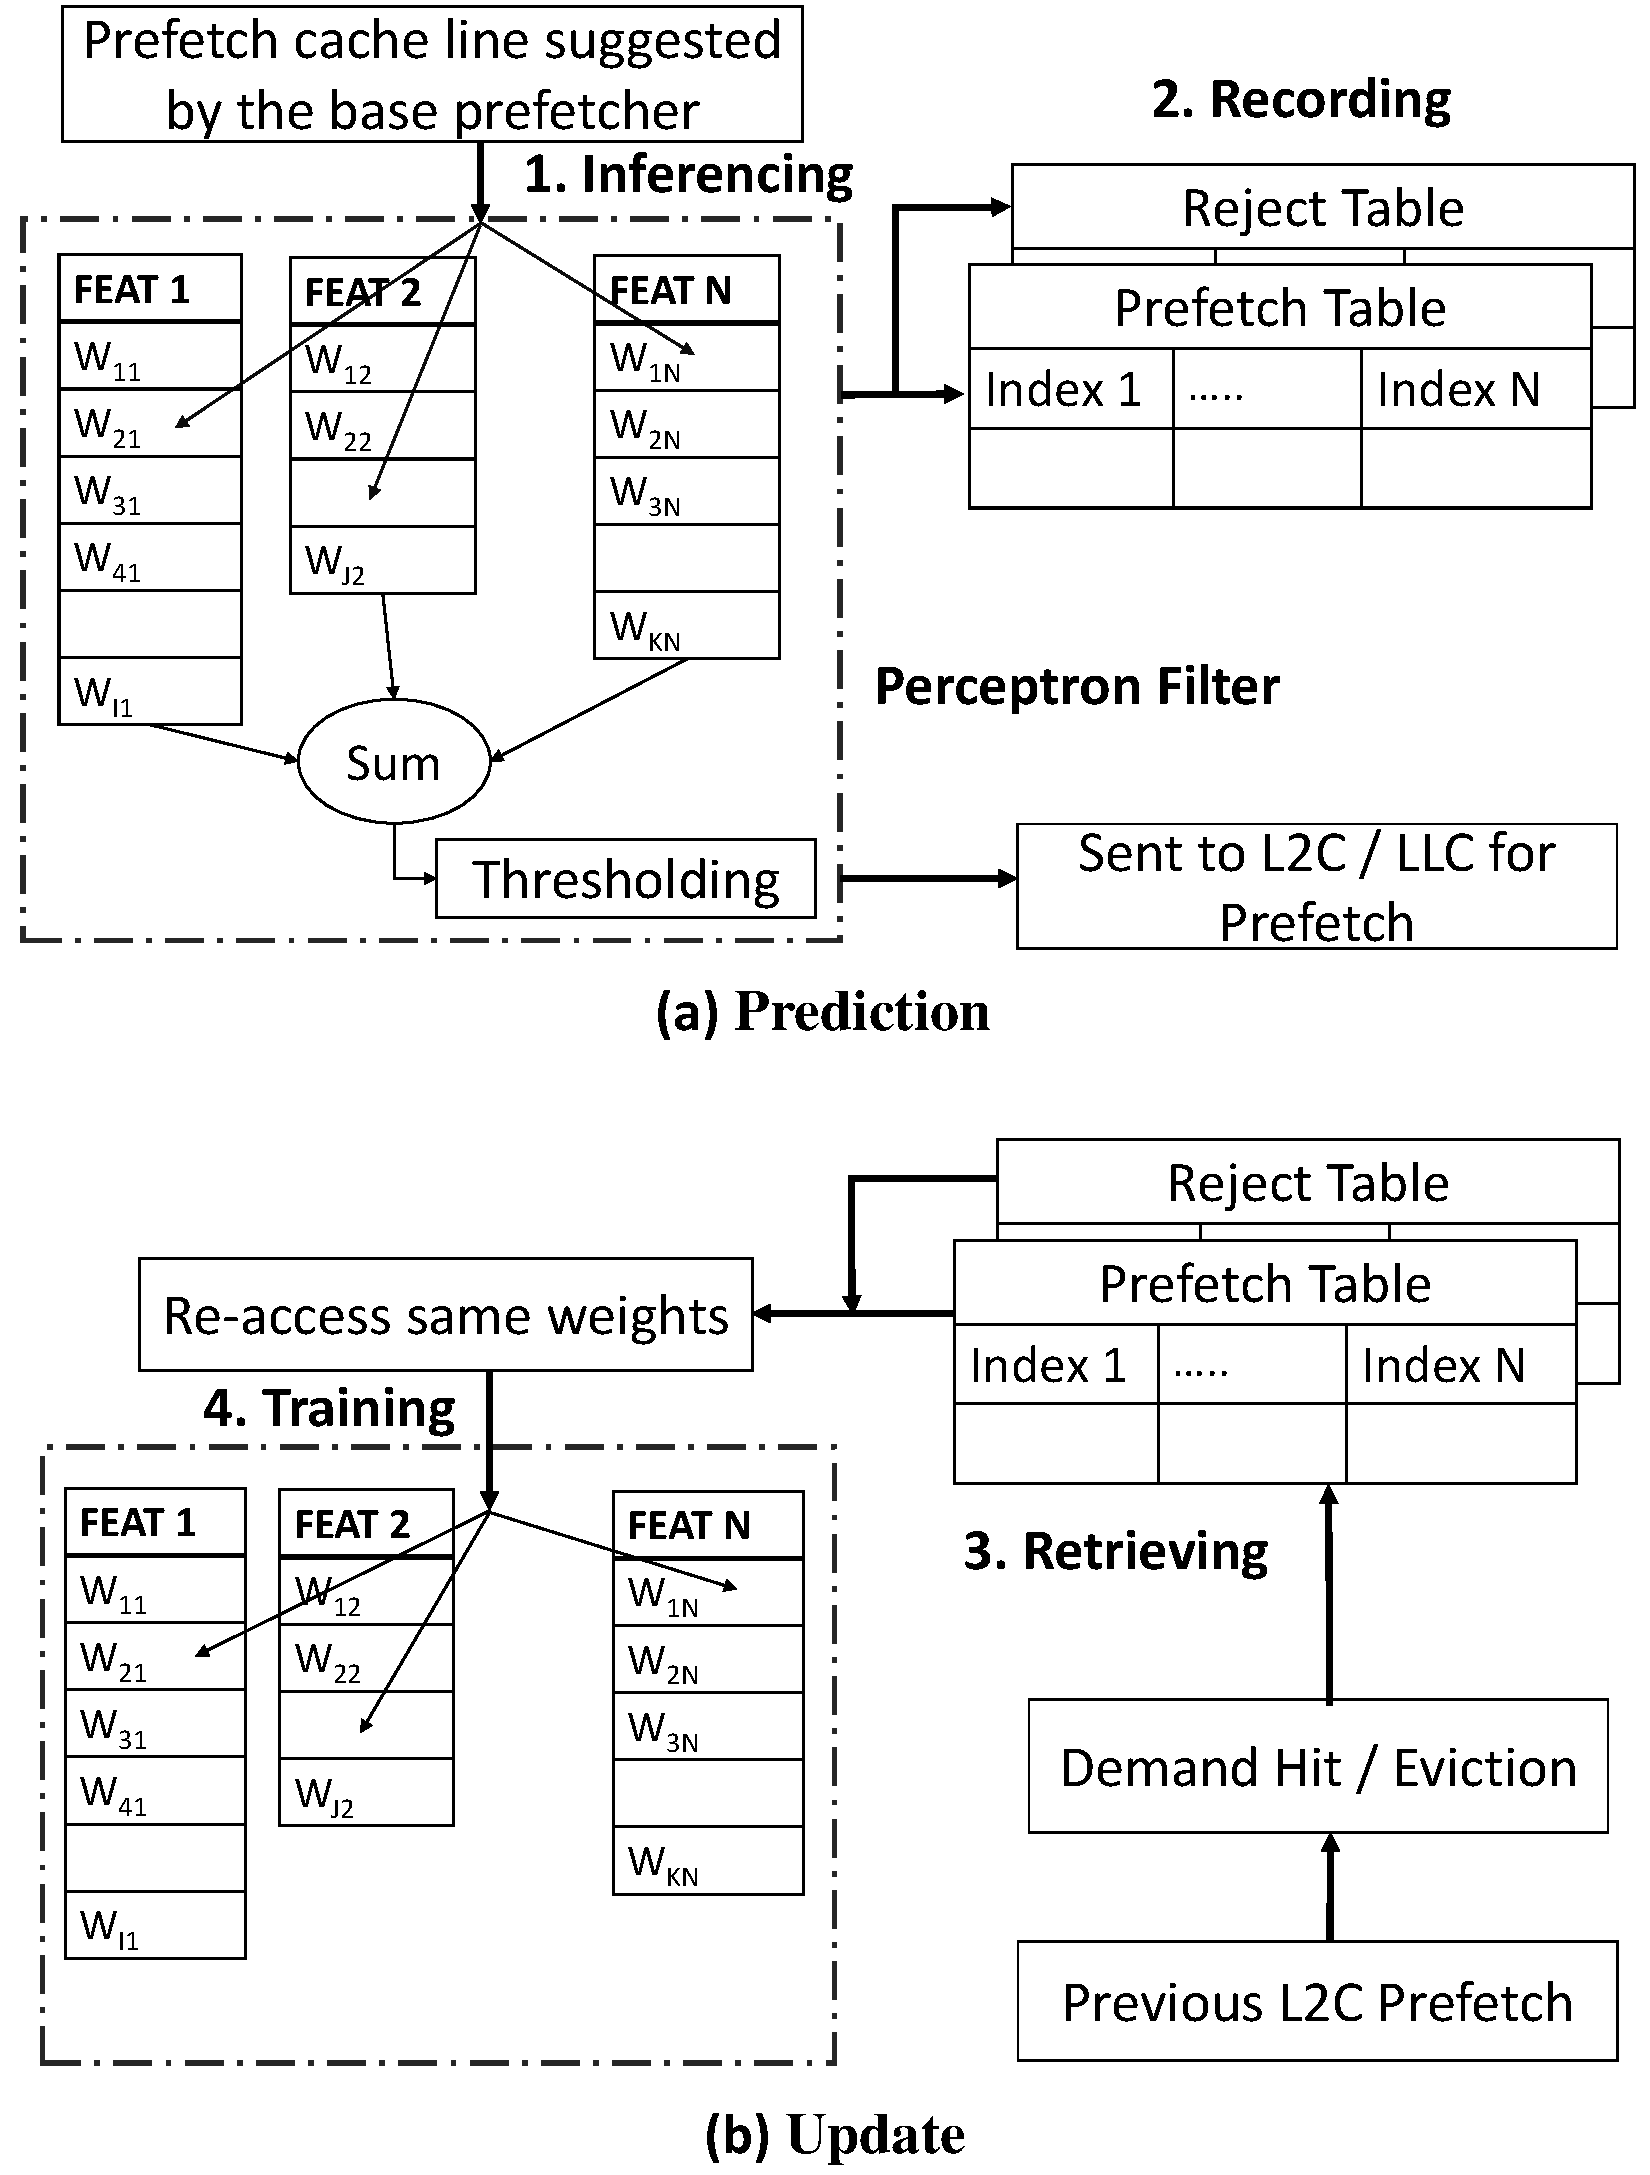
\includegraphics[width=\columnwidth]{Datapath_Separate}
  \caption{PPF Data Path and Operation}
  \label{fig:PPF_Datapath}
  \end{center}
\end{figure}

\subsection{The Perceptron Filter}
\label{Arch-Perceptron}

Figure~\ref{fig:PPF_Datapath} shows the microarchitecture of PPF, as
well as the steps required to filter out not-useful prefetches. The
perceptron filter is organized as a set of tables, where each entry in
the tables holds a \textit{weight}.  For a configuration of PPF using
$N$ number of features, $N$ different tables of weights are needed.
Each feature is used to index a distinct table. The number of entries
of each table varies according to the corresponding feature, hence,
different number of bits are needed to index different tables. Each
weight is a 5-bit saturating counter ranging from -16 to +15. We found
that having 5-bit weights provides a good trade-off between accuracy
and area. A detailed explanation of the storage overhead of PPF can
be found in Section~\ref{Method-Overheads}.
%
\newline
\newline
\noindent \textbf{Inferencing}\\
The {prefetcher} is triggered on every demand access to the L2
Cache, as seen in Figure~\ref{fig:PPF_Hierarchy}.  At this point, 
it has the opportunity to trigger a prefetch.
If it does so, it will also need to decide how many cache blocks to
prefetch.  These blocks can be either placed in the L2 or L3 cache
according to the confidence of the prefetching mechanism.  Once the
{underlying} prefetcher is triggered, the suggested prefetch candidates are
fed to the perceptron filter to determine the usefulness of these
prefetches. The filter ultimately decides whether to issue the
prefetch suggestions of the {underlying} prefetcher. As shown in step 1
of Figure~\ref{fig:PPF_Datapath}(a), to make the decision,
each feature corresponding to a suggested prefetch is used to index a
table and all the corresponding weights are summed. The sum denotes
the confidence value for the suggested prefetch, and is thresholded
against two different values: $\tau_{hi}$ and $\tau_{lo}$.

Prefetches whose sum exceeds $\tau_{hi}$ are placed into the L2 cache.
The higher confidence value hints the prefetch would be useful and
should be prioritized.  A prefetch for which the features result in a
confidence value between $\tau_{lo}$ and $\tau_{hi}$ is allocated in
the larger LLC, as the filter is moderately confident of the future
reuse of the cache block, but not enough to possible pollute a
significantly smaller L2.  Suggested prefetches for which the features
lead to a confidence value lower than $\tau_{lo}$ are not prefetched,
as the low confidence value represents that the perceptron learned
that a similar set of features are associated with non-useful
prefetches.
\newline
\newline
\noindent \textbf{Recording}\\
As shown in step 2 of Figure~\ref{fig:PPF_Datapath}(a) the prefetches
that make it through the inference stage are recorded in the
``Prefetch Table''. The prefetch table is a 1,024-entry, direct mapped
structure that contains all metadata required to re-index the
perceptron entries for training. {Ten bits of the address are 
used to index into the tables, and another six bits are stored to 
perform tag matching.} 

In addition to the prefetch table mentioned above, PPF also maintains
a 1,024-entry direct-mapped ``Reject Table.'' If a prefetch suggestion
is rejected by the perceptron layer, it is logged into the reject
table. The table is used to train the perceptron to avoid false
negatives \textit{i.e.}, cases where the prediction suggested to
reject the prefetch but the prefetch was proven to be useful based on
the observed demand accesses to the L2.
\newline
\newline
\noindent \textbf{Feedback and Data Retrieval}\\
As depicted in step 3, when there is an eviction or a demand access 
to the L2, training for both the {underlying} prefetcher 
and our filter mechanism is triggered. The address of the cache block 
that triggered the training is used to index both the Prefetch and 
Reject tables. {If it is a match, the corresponding
features are retrieved to index into the tables of perceptron weights.}
%
\newline
\newline
\noindent \textbf{Training}\newline As can be seen in step 4 of, 
the address from the demand
request triggering the training is looked up in both tables. If the
address is in the prefetch table and marked as valid, this hints the
previous prediction was correct and this is a useful prefetch. We
compute the sum of the corresponding weights. If the sum falls below a
specific threshold, training occurs and the corresponding weights are
adjusted accordingly. These thresholds are introduced in order to
avoid over-training, helping the filter adapt quickly to changes in
memory behavior. These thresholds are referred to as $\theta_p$ and
$\theta_n$, respectively for the positive and negative values of
training saturation.

On a cache block eviction, we look up the corresponding address in the
prefetch table. If there is a valid entry with this address, the
filter made a misprediction. The block was allocated in the L2 with a
prefetch request that the filter should have categorized as a useless
prefetch. Thus, the corresponding features of the prefetch request are
used to re-index the tables of weights, and those weights are adjusted
accordingly.

Parallel to accessing the prefetch table, on a demand access, the
reject table is accessed. Before the demand access triggers the next
set of prefetches, the reject table is checked for a valid entry. A
hit means that the corresponding cache block was initially suggested
by the {underlying} prefetcher, but wrongly rejected by the perceptron
filter. The perceptron filter learns from this and makes use of the
corresponding features associated to the original prefetch request,
which are stored in the reject table, to index the weights tables and
adjust the weights accordingly.
The implementation of the reject table, allows us to capture the 
information of prefetches that were rejected, and that can be used 
to further optimize our prefetching mechanism.

\subsection{Optimizing PPF for a Given Prefetcher}
\label{Arch-Generalizing}
The above discussion of PPF shows that it is highly modular and can be
adapted to be used over any {underlying} prefetcher for increased prefetch
accuracy. As a first step, all the prefetch
candidates of the prefetcher have to pass through the perceptron filter. 
If qualified, the metadata for perceptron indexing has to be stored. 
Next, when the feedback of a prior prefetch is available in form
of a subsequent demand hit or cache eviction, the stored
metadata needs to be retrieved to update the state of the perceptrons.

\noindent In general, PPF can be adapted to a {new prefetcher} with only a
few modifications:
\newline
\newline
\noindent \textbf{Making the {Underlying} Prefetcher More Aggressive:} By Tuning 
down any internal thresholds or throttling mechanisms to increase its
aggressiveness.
\newline
\newline
\noindent \textbf{Inferencing and Storing:} All prefetch
recommendations are tested using the perceptron inferencing algorithm.
The perceptron's output, \textit{true} or \textit{false}, should be
saved appropriately, along with all metadata required for perceptron
indexing.
\newline
\newline
\noindent \textbf{Retrieving and Training:} When feedback for a
prefetch becomes available, the previously stored metadata can be used
to re-index into the perceptron entries and increment or decrement the
weights.
\newline
\newline
\noindent \textbf{Feature Selection:} Perceptrons essentially
integrate contributions from different features to get a single sum
representing the final confidence.  Thus, perceptron learning can only
be as good as the set of features chosen.  Interestingly, this is what
makes perceptron learning scalable, as it can easily learn to
incorporate newer information in the form of new features.  Some of
the features we developed use information derived directly from
program execution, agnostic to the {underlying} prefetcher.  Beyond that,
the feature set can be expanded to convey any useful information or
metadata available in the {underlying} prefetcher itself.
\newline
\newline
\noindent \textbf{Using Metadata from the Prefetcher:} Some of the 
internal counters specific to the underlying prefetcher can be suitable candidates
for the perceptron features. To make sure that the perceptron layer sees that, 
the relevant metadata must be exported from the prefetcher to PPF. This way,
PPF can be optimized to work tightly-knit with the {underlying} prefetcher.
